\documentclass[12pt, a4paper]{article}
\usepackage{graphicx} % Required for inserting images
\graphicspath{{images/}{images-desafios/}}
\usepackage[a4paper, total={7.5in, 10in}]{geometry}
\usepackage{float} % pra conseguir usar o \begin{figure}[H]
\usepackage{indentfirst} % pra fazer tab n 1 paragrafos dos capitulos
% package pra tabela
\usepackage{multirow}
\usepackage{array}

%pacote pra codigo
\usepackage{listings} 
\usepackage{xcolor}
\definecolor{codegreen}{rgb}{0,0.6,0}
\definecolor{codegray}{rgb}{0.5,0.5,0.5}
\definecolor{codepurple}{rgb}{0.58,0,0.82}
\definecolor{backcolour}{rgb}{0.95,0.95,0.92}

\lstdefinestyle{myCodeStyle}{
	backgroundcolor=\color{backcolour},   
	commentstyle=\color{codegreen},
	keywordstyle=\color{cyan},
	numberstyle=\tiny\color{codegray},
	stringstyle=\color{codepurple},
	basicstyle=\ttfamily\footnotesize,
	breakatwhitespace=false,         
	breaklines=true,                 
	captionpos=b,                    
	keepspaces=true,                 
	%numbers=left,                    
	numbersep=5pt,                  
	showspaces=false,                
	showstringspaces=false,
	showtabs=false,                  
	tabsize=2
}
\lstset{style=myCodeStyle}
\renewcommand{\lstlistingname}{Código}%Muda o termo "Listing":  Listing -> Código
\renewcommand{\lstlistlistingname}{Lista de \lstlistingname s}% List of Listings -> Lista de Códigos


\newcommand{\unit}[1]{\ensuremath{\, \mathrm{#1}}} % comando pra tirar do math mode a unidade de medida

\def\tamanhoGrafico{0.8}

\newcommand{\ohm}{\unit{\Omega} }
\newcommand{\kohm}{\unit{k\Omega}}

\title{
	Laboratório Digital A - PCS3335
	\\ Relatório da Experiência 9
}

\author{
	Alunos:
	\\ Rafael Hipólito Rodrigues - N.USP: 14604308
	\\ {{PERSON-2}} - N.USP: {{PERSON-ID-2}}
	\\ \\
	Turma 3 - Bancada A6
	\\ Professor: Bruno de Carvalho Albertini
}

%\date{}

\begin{document}
	
	\maketitle
	
	\section*{Planejamento: Elaboração do Projeto} 
	
	Nessa experiência começamos a elaborar o projeto da disciplina seguindo o cronograma apresentado na proposta
	de projeto. O objetivo dessa experiência era elabora um circuito que utilizasse o teclado de membrana matricial.
	O teclado de membrana utilizado foi disponibilizado pelo Lab. Dig..
	
	 \begin{figure}[H]
	 	\centering
	 	\includegraphics[width=0.4\linewidth]{images/teclado_matricial_membrana_4x4.jpg}
	 	\caption{Teclado de membrana matricial 4x4 similar ao utilizado.}
	 	\label{fig:teclado_matricial_membrana_4x4}
	 \end{figure}
	 
	 Os objetivos eram:
	 
	 \begin{itemize}
	 	\item Montar o mapa das ligações de linha e coluna do teclado de membrana utilizado.
	 	
	 	\item Elaborar um circuito que ao apertar um botão do teclado, o seu valor era mostrado no display de 
	 	7 segmentos
	 \end{itemize}
	
	\section*{Resultados}
	
	Apos testar o teclado o grupo conseguiu montar um mapa das ligações de linha e coluna do teclado.
	
	\begin{figure}[H]
		\centering
		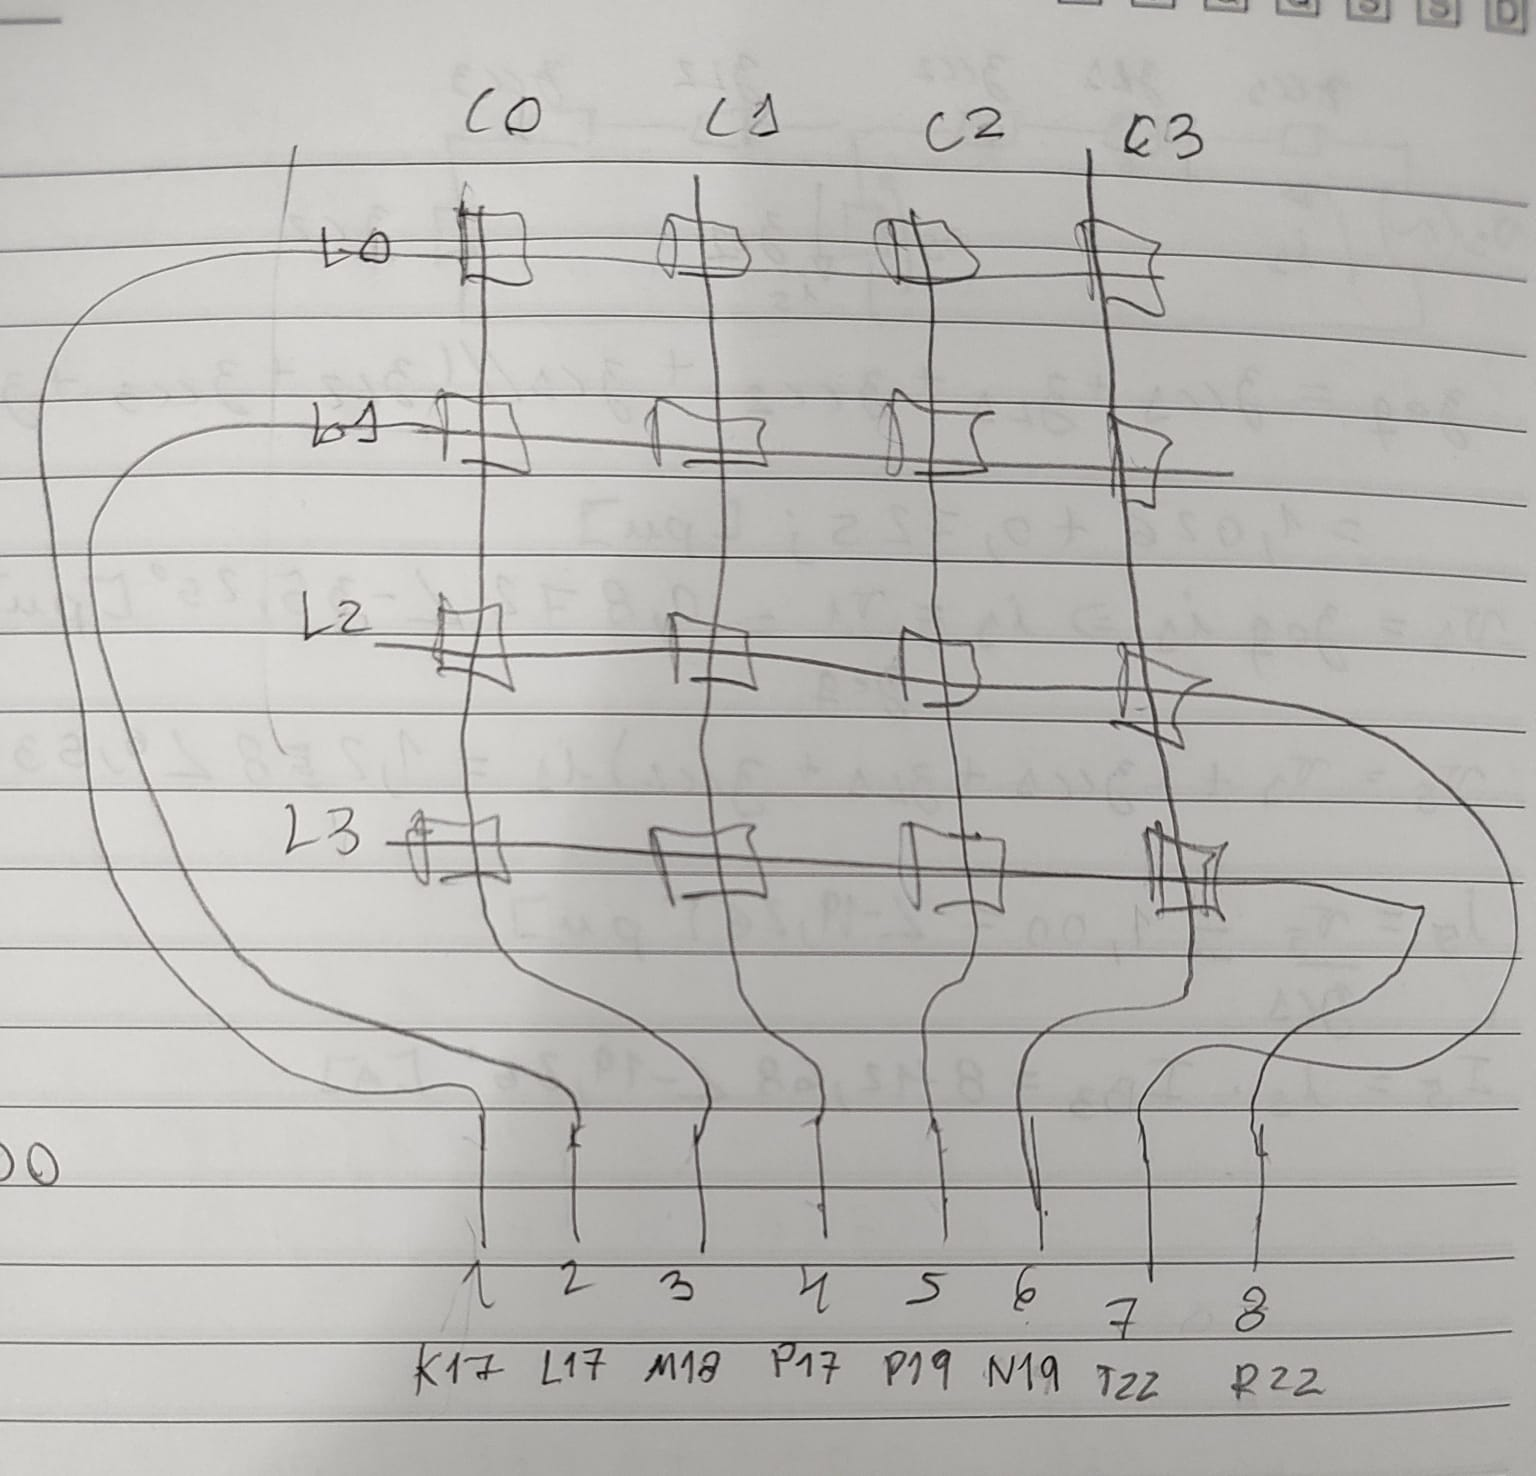
\includegraphics[width=0.7\linewidth]{images/mapa.jpeg}
		\caption{Esquema de mapa montado pelo grupo.}
		\label{fig:mapa}
	\end{figure}
	
	Assim o grupo conseguiu elaborar um circuito que reconhecesse qual tecla estava sendo pressionada.
	
	\begin{figure}[H]
		\centering
		\includegraphics[width=0.9\linewidth]{images/RLT.png}
		\caption{RLT do circuito elaborado pelo grupo.}
		\label{fig:mapa}
	\end{figure} 
	
	Assim o próximo passo do projeto é elaborar um circuito que utilize o teclado para armazenar valores uma memoria.
	
	
\end{document}
